Chương này tập trung làm rõ hành vi của chương trình, độ tương tự về
hành vi giữa hai chương trình và các phương pháp đo độ tương tự về
hành vi, sẽ được trình bày trong Phần \ref{sec:behavior} và
\ref{sec:metrics}. Ngoài ra, chương này còn trình bày một số kiến thức
cơ sở về kiểm thử phần mềm, các phương pháp kiểm thử phần mềm, kỹ
thuật sinh dữ liệu kiểm thử trong Phần \ref{sec:base}.

\section{Kiến thức cơ sở}
\label{sec:base}

Ý tưởng chính của việc đo độ tương tự về hành vi giữa hai chương trình
máy tính là dựa trên tập dữ liệu vào, đếm số lượng dữ liệu ra tương
ứng giống nhau giữa hai chương trình và đo tỷ lệ tương tự. Dữ liệu vào
phải được chọn sao cho phủ nhiều nhất miền vào của chương trình. Về cơ
bản, độ tương tự này được đo dựa trên dữ liệu các ca kiểm thử. Chương
này trình bày ngắn gọn về kiểm thử phần mềm cùng việc sinh dữ liệu
kiểm thử, chủ yếu tập trung vào phương pháp thực thi biểu trưng một
chương trình (\emph{DSE -- Dynamic Symbolic Execution}) nhằm giúp tăng độ phủ
của dữ liệu thử.

\subsection{Kiểm thử phần mềm}
Hiện nay, ngành công nghiệp phần mềm giữ vai trò hết sức quan trọng, một số nước có nền công nghệ thông tin phát triển thì ngành công nghiệp phần mềm có khả năng chi phối cả nền kinh tế. Vì vậy,  việc đảm bảo chất lượng phần mềm trở nên cần thiết hơn bao giờ hết.

Quá trình phát hiện và khắc phục lỗi của phần mềm là một công việc đòi hỏi nhiều nỗ lực, công sức, phát sinh thêm nhiều chi phí trong việc phát triển phần mềm. Một sản phẩm phần mềm đạt chất lượng cao, đáp ứng được yêu cầu của người sử dụng sẽ được nhiều người biết đến, nó mang lại hiệu quả tích cực trong công việc của người sử dụng. Ngược lại, một phần mềm kém chất lượng sẽ gây thiệt hại về kinh tế, ảnh hưởng đến công việc của người sử dụng. Vì vậy, yêu cầu đặt ra đó là một sản phẩm phần mềm phải đảm bảo được sự ổn định, không phát sinh lỗi trong quá trình sử dụng.

Kiểm thử phần mềm chính là một quá trình hoặc một loạt các quy trình được thiết kế, để đảm bảo mã máy tính chỉ làm những gì nó được thiết kế và không làm bất cứ điều gì ngoài ý muốn \cite{myers2011art}. Phần mềm phải được dự đoán và nhất quán, không gây bất ngờ cho người dùng. Đây là một bước quan trọng trong quá trình phát triển một phần mềm, giúp cho nhà phát triển phần mềm và người sử dụng thấy được hệ thống đã đáp ứng được yêu cầu đặt ra.

\subsubsection{Các phương pháp kiểm thử}

Có nhiều phương pháp để kiểm thử phần mềm, trong đó hai phương pháp
kiểm thử chính là \emph{kiểm thử tĩnh} và \emph{kiểm thử động}.

\emph{Kiểm thử tĩnh (Static testing)} là phương pháp kiểm thử phần mềm
bằng cách duyệt lại các yêu cầu và các đặc tả, mã lệnh chương trình
bằng tay, thông qua việc sử dụng giấy, bút để kiểm tra tính logic từng
chi tiết mà không cần chạy chương trình. Kiểu kiểm thử này thường được
sử dụng bởi chuyên viên thiết kế, người viết mã lệnh chương
trình. Kiểm thử tĩnh cũng có thể được tự động hóa bằng cách thực hiện
kiểm tra toàn bộ hệ thống thông qua một trình thông dịch hoặc trình
biên dịch, xác nhận tính hợp lệ về cú pháp của chương trình.
		
\emph{Kiểm thử động (Dynamic testing)} là phương pháp kiểm thử thông
qua việc thực thi chương trình để kiểm tra trạng thái tác động của
chương trình, dựa trên các ca kiểm thử xác định các đối tượng kiểm thử
của chương trình. Đồng thời, kiểm thử động sẽ tiến hành kiểm tra cách
thức hoạt động của mã lệnh, tức là kiểm tra phản ứng từ hệ thống với
các biến thay đổi theo thời gian. Trong kiểm thử động, phần mềm phải
được biên dịch và chạy, và bao gồm việc nhập các giá trị đầu vào và
kiểm tra giá trị đầu ra có như mong muốn hay không.

Trong luận văn này, độ tương tự về hành vi giữa hai chương trình được
đo thông qua việc thực thi hai chương trình, tức là sử dụng phương
pháp kiểm thử động.
	
\subsubsection{Các chiến lược kiểm thử}

Hai chiến lược kiểm thử phần mềm được sử dụng nhiều nhất đó là \emph{kiểm thử hộp đen} và \emph{kiểm thử hộp trắng}.
	
\emph{Kiểm thử hộp đen – Black box} là một chiến lược kiểm thử với
cách thức hoạt động chủ yếu dựa vào hướng dữ liệu inputs/outputs của
chương trình, xem chương trình như là một ``hộp đen''. Chiến lược kiểm
thử này hoàn toàn không quan tâm về cách xử lý và cấu trúc bên trong
của chương trình, nó tập trung vào tìm các trường hợp mà chương trình
không thực hiện theo các đặc tả. Tuy nhiên, phương pháp kiểm thử này
cũng có mặt hạn chế của nó, kiểm thử viên không biết các phần mềm cần
kiểm tra thực sự được xây dựng như thế nào, cố gắng viết rất nhiều ca
kiểm thử để kiểm tra một chức năng của phần mềm nhưng lẽ ra chỉ cần
kiểm tra bằng một vài ca kiểm thử, hoặc một số phần của chương trình
có thể bị bỏ qua không được kiểm tra.

Do vậy, kiểm thử hộp đen có ưu điểm là đánh giá khách quan, mặt khác
nó lại có nhược điểm là thăm dò mù. Trong phần nghiên cứu của đề tài,
kiểm thử hộp đen cũng được sử dụng như một phương pháp đo độ tương tự
hành vi của các chương trình.
		
\emph{Kiểm thử hộp trắng – White box} là một chiến lược kiểm thử khác,
trái ngược hoàn toàn với kiểm thử hộp đen, còn gọi là kiểm thử hướng
logic của phần mềm. Cách kiểm thử này cho phép tạo ra dữ liệu thử
nghiệm từ việc kiểm tra, khảo sát cấu trúc bên trong và kiểm thử tính
logic của chương trình. Dữ liệu thử nghiệm có độ phủ lớn, đảm bảo tất
cả các đường dẫn, hoặc các nhánh của chương trình được thực hiện ít
nhất một lần, khắc phục được những nhược điểm thăm dò mù trong cách
kiểm thử hộp đen.			

\subsection{Kỹ thuật Dynamic symbolic execution}
\label{sec:dse}

Dynamic symbolic execution (DSE) là một kỹ thuật duyệt tự động tất cả các đường đi có thể của chương trình bằng cách chạy chương trình với nhiều giá trị đầu vào khác nhau để tăng độ phủ của dữ liệu thử \cite{xie2009fitness}.

Dựa trên kiểu dữ liệu các tham số đầu vào của chương trình, DSE sẽ tạo ra các giá trị đầu vào cụ thể và thực thi chương trình với các giá trị cụ thể vừa tạo. Trong quá trình thực thi, DSE sẽ ghi nhận lại ràng buộc tại các nút rẽ nhánh của chương trình, phủ định lại các ràng buộc này và sinh các giá trị đầu vào thỏa các điều kiện ràng buộc vừa được ghi nhận. Với một giá trị đầu vào cụ thể, DSE sẽ thực thi chương trình và duyệt được một đường đi cụ thể, quá trình thực thi này sẽ lặp lại cho đến khi duyệt hết tất cả các đường đi của chương trình. Từ đó, chúng tôi xây dựng Thuật toán \ref{alg:DSE} để mô tả cách thức hoạt động tạo tập dữ liệu đầu vào thử nghiệm của kỹ thuật DSE.

\begin{algorithm}
	\caption{Dynamic symbolic execution}
	\label{alg:DSE}
	\begin{algorithmic}
		\item $ P $: Chương trình được thực thi		
		\item $ I $: Tập đầu vào của $ P $		
		\item $ P(i)$: Thực thi $ P $ với $ i \in I  $
		\item $ J $: Tập các giá trị được thực thi trên $ P $, ký hiệu $ J = \{i | P(i)\} $
		\item $ Q $: Tập các ràng buộc của $ P $, hay còn gọi là tập các điều kiện đường đi của $ P $
		\item $ C(i) $: Là ràng buộc thu gom được từ việc thực thi $ P(i)$
		\item $ C'(i) $: Là điều kiện đường đi suy ra từ $ C(i) $
        \item Set $J:= \varnothing $
        \item Set $i:= Random(I) $; 
        \item loop 
        	\subitem Set $ Q:= \varnothing $
        	\subitem Chọn đầu vào $ i \notin J $
        	\Comment{Dừng lại nếu $ i \in J $}         	
          	\subitem Thực thi P(i) 
          	\subitem Lưu lại điều kiện đường đi $ C(i) $ vào $ Q $; suy ra $ C'(i)$ 
	        \subitem Từ $ Q $ và $ C'(i) $ suy ra $ i $
          	\subitem Set J := J $\cup $ i
        \item end loop
	\end{algorithmic}
\end{algorithm}

Để hiểu rõ cách thức hoạt động tạo tập dữ liệu đầu vào thử nghiệm của kỹ thuật DSE chúng ta phân tích ví dụ trong Hình \ref{lst:vddse} \cite{DSE}, với hàm \texttt{test\_me} có hai tham số đầu vào là \texttt{int x} và \texttt{int y} và hàm này không có giá trị trả về.

\begin{figure}[H]
	\centering
	\label{lst:vddse}
	\lstinputlisting[caption={Ví dụ minh họa cách thức hoạt động của kỹ thuật DSE},label={DSE}]{DSE.cs}	
\end{figure}	

Đầu tiên, DSE tạo hai đầu vào có giá trị ngẫu nhiên, giả sử $x = 22$ và $y = 7$. Đồng thời, DSE theo dõi trạng thái biểu trưng của chương trình với $ x $ bằng một số $x_{0}$ và $ y $ bằng một số $y_{0}$ (Hình \ref{fig:dse11}).

\begin{figure}[H]	
	\begin{center}
		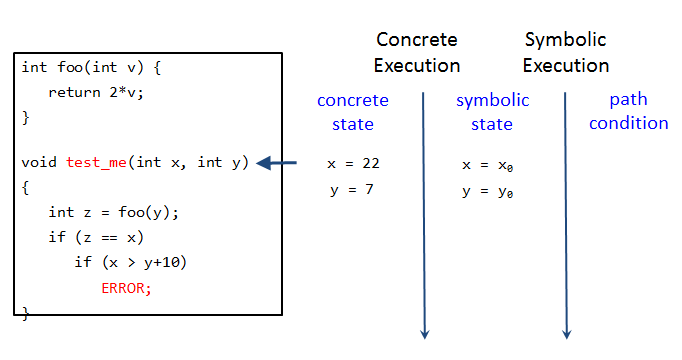
\includegraphics[scale=.7]{dse11.png}
	\end{center}
	\caption{DSE tạo hai đầu vào có giá trị ngẫu nhiên}
	\label{fig:dse11}	
\end{figure}

Ở dòng đầu tiên, số nguyên $ z $ được gán bằng hàm $ foo(y) $, nghĩa là số nguyên $ z = 14 $ và ở trạng thái biểu trưng của số nguyên $ z $ bằng $ 2*y_{0} $ (Hình \ref{fig:dse12}).

\begin{figure}[H]	
	\begin{center}
		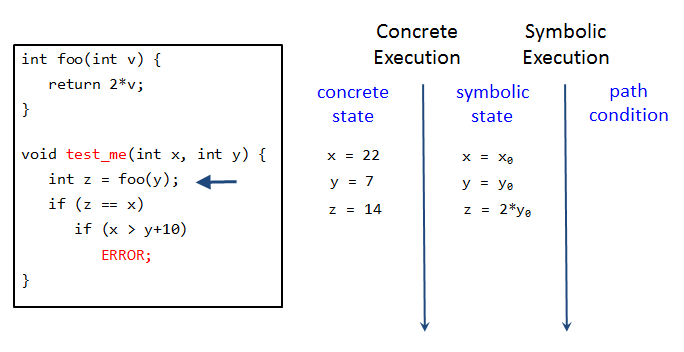
\includegraphics[scale=.7]{dse12.png}
	\end{center}
	\caption{DSE gán số nguyên $ z $ bằng hàm $foo(y)$}
	\label{fig:dse12}	
\end{figure}

Tại điểm nhánh $z == x$, DSE nhận thấy giá trị của $ z $ và $ x $ không bằng nhau. Về mặt biểu trưng, DSE lưu lại ràng buộc $ z != x $ như là điều kiện đường dẫn của chương trình với các giá trị biểu trưng của $ z $ và $ x $ là $ 2*y_{0} != x_{0} $. Sau đó, DSE đi theo đi theo nhánh $ fasle $, dẫn đến kết thúc chương trình (Hình \ref{fig:dse13}).

\begin{figure}[H]	
	\begin{center}
		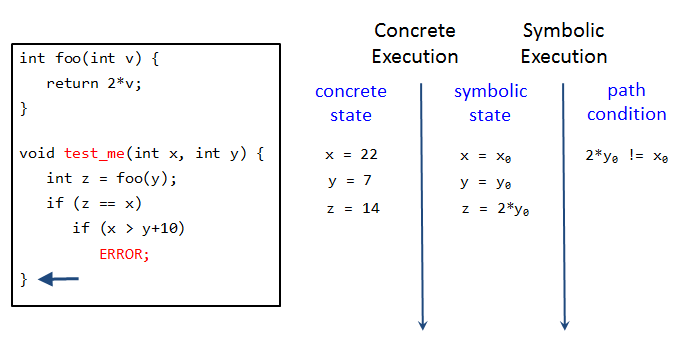
\includegraphics[scale=.7]{dse13.png}
	\end{center}
	\caption{DSE lưu lại ràng buộc $ z != x $ của chương trình  }
	\label{fig:dse13}	
\end{figure}

Lúc này, DSE quay trở lại điểm nhánh $z == x$ và chọn nhánh $ true $. Để thực hiện việc này, DSE phủ định lại ràng buộc trong điều kiện đường dẫn $2*y_{0} != x_{0}$ thành $2*y_{0} == x_{0}$. Sau đó, DSE thực hiện giải ràng buộc $2*y_{0} == x_{0}$ và trả về hai số nguyên thỏa ràng buộc có giá trị $ x_{0} = 2$, $ y_{0} = 1 $ (Hình \ref{fig:dse2}).

\begin{figure}[H]	
	\begin{center}
		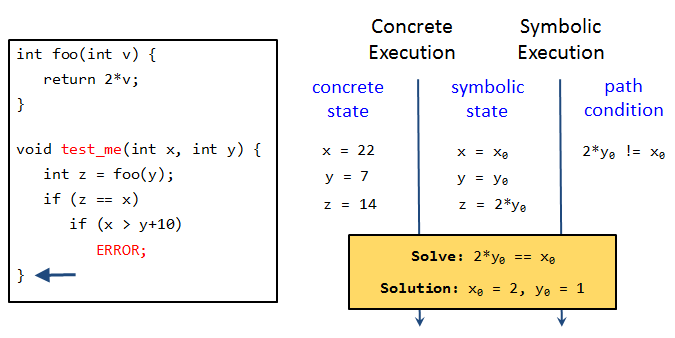
\includegraphics[scale=.7]{dse2.png}
	\end{center}
	\caption{DSE tính toán và giải ràng buộc $2*y_{0} == x_{0}$}
	\label{fig:dse2}	
\end{figure}

Sau khi có hai số nguyên thỏa ràng buộc của chương trình, DSE khởi động lại hàm $ test\_me $ với các giá trị đầu vào cụ thể $x = 2$, $y = 1$ vừa tạo ra trước đó và tiếp tục theo dõi trạng thái biểu trưng của chương trình với $ x $ bằng một số $x_{0}$ và $ y $ bằng một số $y_{0}$ (Hình \ref{fig:dse21}).

\begin{figure}[H]	
	\begin{center}
		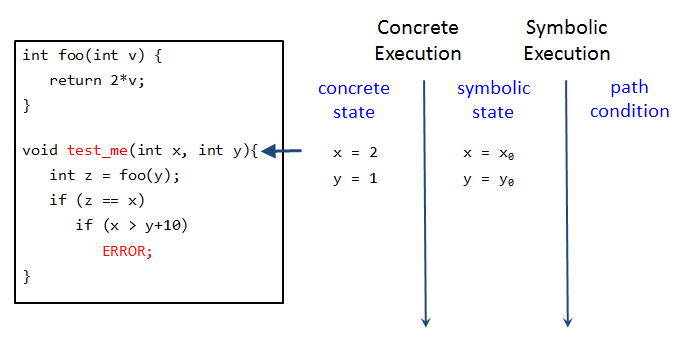
\includegraphics[scale=.7]{dse21.png}
	\end{center}
	\caption{DSE khởi động lại hàm \texttt{test\_me}}
	\label{fig:dse21}		
\end{figure}

Sau khi thực hiện dòng đầu tiên, biến $ z $ sẽ có giá trị bằng $2$ (đầu ra của hàm $ foo(y) $) và DSE lưu giá trị biểu trưng của số nguyên $ z $ là $z = 2*y_{0}$ (Hình \ref{fig:dse22}).

\begin{figure}[H]	
	\begin{center}
		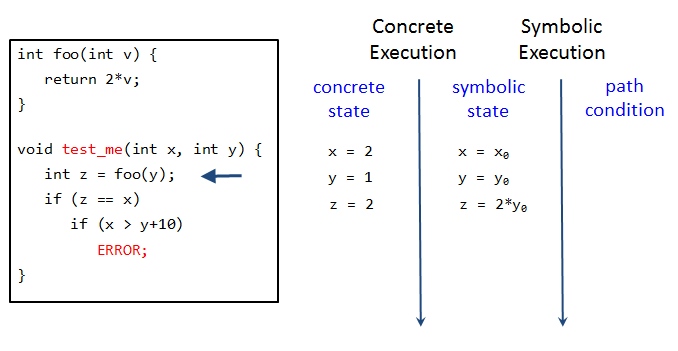
\includegraphics[scale=.7]{dse22.png}
	\end{center}
	\caption{DSE lưu giá trị biểu trưng của số nguyên $ z $}
	\label{fig:dse22}		
\end{figure}

Tại điểm nhánh $ z == x $, DSE thấy giá trị của biến $ z == x $, đây là điều kiện $ true $ nên DSE lưu lại ràng buộc trong điều kiện đường dẫn là $2*y_{0} == x_{0}$. Sau đó DSE tiếp tục kiểm tra các dòng tiếp theo của nhánh $ true $ (Hình \ref{fig:dse23}).

\begin{figure}[H]	
	\begin{center}
		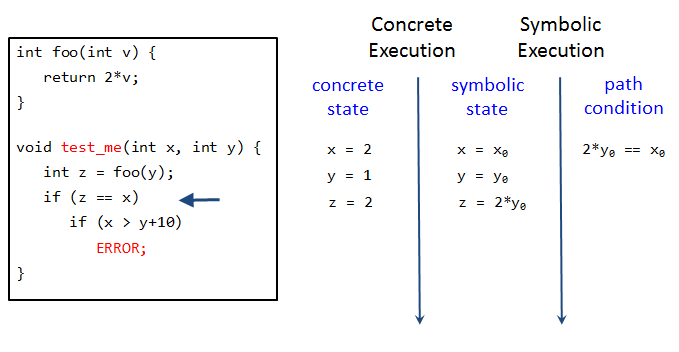
\includegraphics[scale=.7]{dse23.png}
	\end{center}
	\caption{DSE ghi nhận điều kiện ràng buộc $2*y_{0} == x_{0}$}
	\label{fig:dse23}	
\end{figure}

Tại điểm nhánh tiếp theo $ x > y+10 $, lúc này $ x $ có giá trị bằng $2$, $(y + 10)$ có giá trị bằng $11$ nên DSE chọn nhánh $ fasle $ và kết thúc chương trình. Cùng lúc đó, DSE lưu lại ràng buộc trong điều kiện đường dẫn của chương trình là $x_{0} <= y_{0} + 10$ (Hình \ref{fig:dse24}).

\begin{figure}[H]	
	\begin{center}
		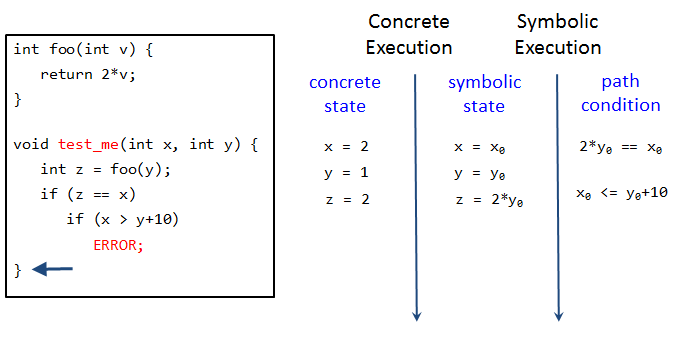
\includegraphics[scale=.7]{dse24.png}
	\end{center}
	\caption{DSE lưu lại ràng buộc $x_{0} <= y_{0} + 10$}
	\label{fig:dse24}		
\end{figure}

Vì đã đến cuối chương trình nên DSE quay lại điểm nhánh $ x > y+10 $ và thực hiện phủ định lại ràng buộc $x_{0} <= y_{0} + 10$ thành $ x_{0} > y_{0} + 10 $. Sau đó, DSE thực hiện giải ràng buộc $(2*y_{0} == x_{0}) and (x_{0} > y_{0} + 10)$ và trả về giá trị $x_{0} = 30$ và $y_{0} = 15$ (Hình \ref{fig:dse3})

\begin{figure}[H]	
	\begin{center}
		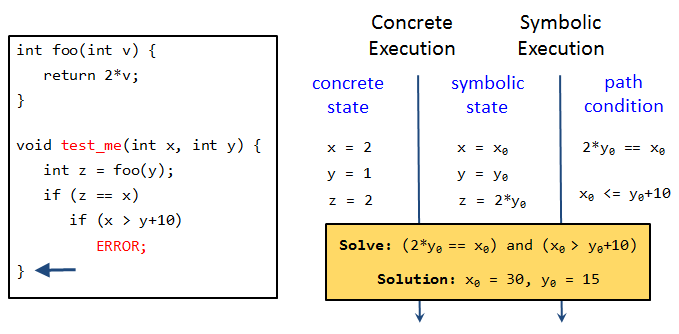
\includegraphics[scale=.7]{dse3.png}
	\end{center}
	\caption{DSE thực hiện giải ràng buộc $(2*y_{0} == x_{0}) and (x_{0} > y_{0} + 10)$}
	\label{fig:dse3}
\end{figure}

Bây giờ, DSE chạy lại hàm \texttt{test\_me} một lần nữa với đầu vào cụ thể $x = 30$ và $y = 15$ và theo dõi trạng thái biểu trưng của chương trình với $x = x_{0}$ và $y = y_{0}$ (Hình \ref{fig:dse31})

\begin{figure}[H]	
	\begin{center}
		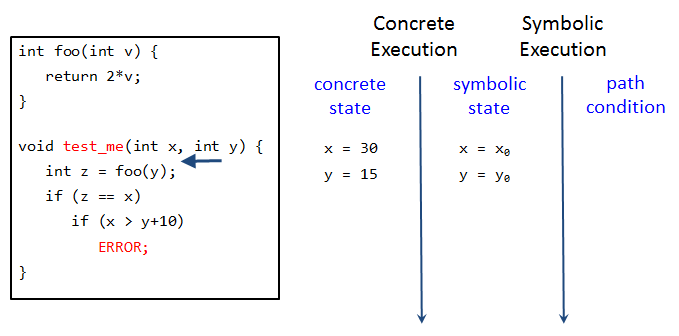
\includegraphics[scale=.7]{dse31.png}
	\end{center}
	\caption{DSE chạy lại hàm \texttt{test\_me} với $ x = 30 $ và $ y = 15 $}
	\label{fig:dse31}
\end{figure}


Ở dòng đầu tiên, số nguyên $ z $ lúc này bằng $ 30 $ và ở trạng thái biểu trưng của chương trình DSE lưu giá trị của số nguyên $ z $ là $ z = 2*y_{0} $ như những lần trước đó (Hình \ref{fig:dse32})

\begin{figure}[H]	
	\begin{center}
		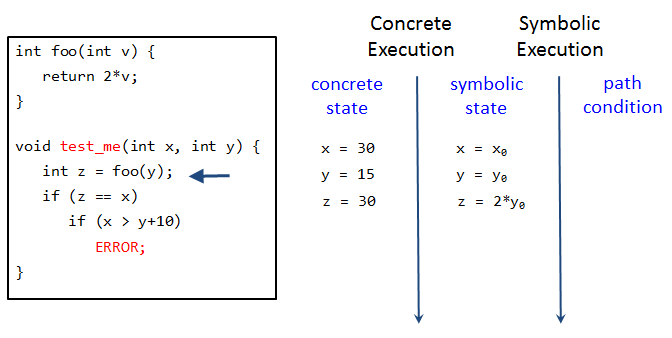
\includegraphics[scale=.7]{dse32.png}
	\end{center}
	\caption{DSE lưu lại trạng thái biểu trưng số nguyên \texttt{z}}
	\label{fig:dse32}
\end{figure}

Tại điểm nhánh $ z == x $, DSE nhận thấy giá trị của $ z $ bằng giá trị của $ x $, đây là điều kiện $ true $ nên DSE thực thi chương trình theo nhánh $ true $, cùng lúc đó DSE lưu lại ràng buộc biểu trưng trong điều kiện đường dẫn của chương trình là $ 2*y_{0} == x_{0} $ cho điểm nhánh này (Hình \ref{fig:dse33})

\begin{figure}[H]	
	\begin{center}
		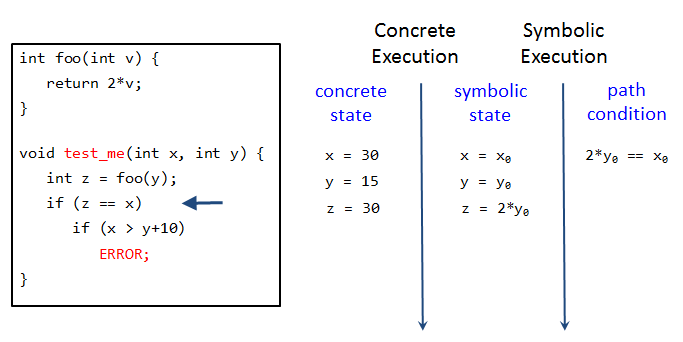
\includegraphics[scale=.7]{dse33.png}
	\end{center}
	\caption{DSE lưu lại điều kiện đường dẫn của chương trình $ 2*y_{0} == x_{0} $}
	\label{fig:dse33}
\end{figure}

Tại điểm nhánh tiếp theo $ x > y+10 $, lúc này giá trị $x = 30 $, $ y = 15 $ nên $ x $ thực sự lớn hơn $(y+10)$, vì vậy DSE thêm một ràng buộc biểu trưng mới là $ x_{0} > y_{0}+ 10 $. Nhánh này dẫn đến $ ERROR $ và kết thúc chương trình nên chúng ta đã xác định được giá trị đầu vào cụ thể làm cho chương trình dẫn đến $ ERROR $ là $x = 30$ và $y = 15$ (Hình \ref{fig:dse4}).

\begin{figure}[H]
	\begin{center}
		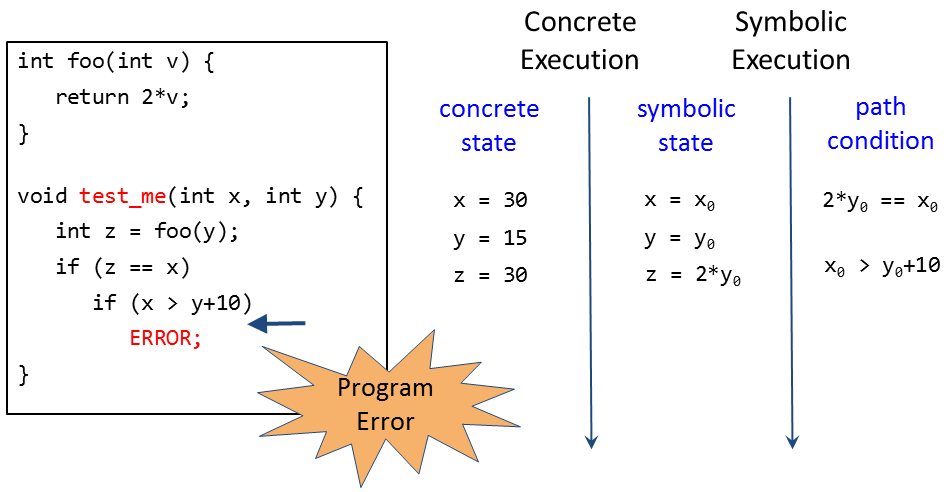
\includegraphics[scale=.6]{dse4.png}
	\end{center}	
	\caption{DSE chạy chương trình với giá trị đầu vào $x = 30$ và $y = 15$}
\label{fig:dse4}
\end{figure}

Với mỗi giá trị đầu vào, DSE thực thi chương trình và duyệt được một đường đi cụ thể. Sau 3 lần thực thi chương trình DSE đã tạo ra được một tập các giá trị đầu vào $[22,7] [2,1] [30,15]$ có thể phủ được tất cả các nhánh trong chương trình.
	
\subsection{Một số công cụ áp dụng DSE}	

Trên thế giới hiện có nhiều công cụ sử dụng kỹ thuật DSE để giải quyết
các ràng buộc và tạo ra các giá trị đầu vào có độ phủ cao như như Pex
\cite{tillmann2008pex} và SAGE \cite{godefroid2008automated}\dots và
những công cụ này được phát triển để có thể chạy được trên nhiều nền
tảng khác nhau. Chúng ta có thể tham khảo một số công cụ khác ở Bảng \ref{tbl:DSETools}.
		
\begin{table}[h]
  \centering
  \label{tbl:DSETools}
  \caption{Một số công cụ áp dụng kỹ thuật DSE}
  \begin{tabular} {|c|c|l|}
    \hline 
    \textbf{Tên Công cụ} & \textbf{Ngôn ngữ} & \textbf{Url} \\ 
    \hline 
    KLEE & LLVM & klee.github.io/ \\ 
    \hline 
    JPF	 & Java	& babelfish.arc.nasa.gov/trac/jpf \\
    \hline 
    jCUTE &	Java &	github.com/osl/jcute \\
    \hline 
    janala2	 & Java &	github.com/ksen007/janala2 \\
    \hline 
    JBSE	& Java	 & github.com/pietrobraione/jbse \\
    \hline 
    KeY &	Java &	www.key-project.org/ \\	
    \hline 
    Mayhem & 	Binary &	forallsecure.com/mayhem.html \\
    \hline 
    Otter &	C	& bitbucket.org/khooyp/otter/overview \\
    \hline 
    Rubyx & 	Ruby &	www.cs.umd.edu/~avik/papers/ssarorwa.pdf \\
    \hline 
    Pex	& .NET Framework	 & research.microsoft.com/en-us/projects/pex/ \\
    \hline 
    Jalangi2 &	JavaScript &	github.com/Samsung/jalangi2 \\
    \hline 
    Kite &	LLVM &	www.cs.ubc.ca/labs/isd/Projects/Kite/ \\
    \hline 
    pysymemu &	x86-64 / Native	 &github.com/feliam/pysymemu/ \\
    \hline 
    Triton	& x86 and x86-64 &	triton.quarkslab.com \\	
    \hline 
    BE-PUM &	x86	 & https://github.com/NMHai/BE-PUM	 \\	
    \hline
  \end{tabular} 
\end{table}
	
\section{Hành vi của chương trình }
\label{sec:behavior}

Trong luận văn này, hành vi của một chương trình là hành động biến đổi
một dữ liệu đầu vào thành đầu ra tương ứng. Chương trình được xem như
một hộp đen. Hành vi biến đổi của chương trình từ đầu vào sang đầu ra
là hành động một bước (\emph{one step action/big step}). Nghĩa là ta
không quan tâm đến sự thay đổi của dữ liệu qua từng bước nhỏ khi thực
hiện mỗi câu lệnh trong chương trình mà chỉ xem xét sự thay đổi qua
một bước lớn, xem tất cả các câu lệnh là một câu lệnh ghép.

Để hình thức hóa hành vi của một chương trình và sử dụng trong những
phần tiếp theo, ta tìm hiểu các định nghĩa hình thức liên quan đến
việc thực thi một chương trình, sự tương đương về hành vi giữa hai
chương trình, sự khác biệt về hành vi và độ tương tự về hành vi giữa
hai chương trình.
        
\subsection{Thực thi chương trình}

Việc thực thi một chương trình có thể xem là sự tương ứng mỗi giá trị vào với một giá trị ra, được nêu ra trong Định nghĩa \ref{def:progexe}.

\begin{definition}[Thực thi chương trình]
  \label{def:progexe}
  Cho $P$ là một chương trình, $I$ là tập hợp các trị đầu vào của $P$
  và $O$ là tập hợp các giá trị đầu ra của $P$. Thực thi chương trình
  P là ánh xạ:
  \[exec: P \times I \rightarrow O.
  \]
\end{definition}

Với giá trị đầu vào $i \in I$, sau khi thực thi chương trình $P$ trên
$i$ ta có giá trị đầu ra tương ứng $o \in O, o = exec(P, i)$.

\subsection{Tương đương về hành vi}

Hai chương trình được gọi là tương đương với nhau về hành vi nếu chúng
biến đổi cùng một giá trị vào thành cùng một giá trị ra đối với mọi
giá trị trên miền vào. Xét ví dụ hai chương trình trong Mã lệnh
\ref{lst:SwitchCase} và \ref{lst:IfElse}.

\begin{minipage}[t]{0.45\linewidth}
  \lstinputlisting[label={lst:SwitchCase}, caption =
  {Sử dụng \texttt{switch...case}}]{SwitchCase.cs}
\end{minipage}%
\hfill\vrule\hfill
\begin{minipage}[t]{0.45\linewidth}
  \lstinputlisting[label={lst:IfElse}, caption =
  {Sử dụng \texttt{if...else}}]{IfElse.cs}
\end{minipage}%

Mã lệnh \ref{lst:SwitchCase} và \ref{lst:IfElse} có cùng tham số đầu vào
\texttt{x} kiểu \texttt{int}, cùng tính toán và trả về giá trị
\texttt{y} phụ thuộc vào \texttt{x} theo cách: nếu \texttt{x = 1} thì
trả về \texttt{y + 4}, nếu \texttt{x = 2} thì trả về \texttt{2y}, còn
không thì trả về giá trị bình phương của \texttt{y}.

Rõ ràng hành vi của hai mã lệnh chương trình trên là tương đương vì
chúng trả về giá trị \texttt{y} giống nhau với cùng mỗi giá trị vào
kiểu số nguyên \texttt{x}, mặc dù chúng có cấu trúc khác nhau (Mã lệnh
\ref{lst:SwitchCase} sử dụng cấu trúc \texttt{switch...case}, Mã lệnh
\ref{lst:IfElse} sử dụng cấu trúc \texttt{if...else} để kiểm tra giá
trị đầu vào $x$). Sự tương đương về hành vi của hai chương trình được
hình thức hóa trong Định nghĩa \ref{def:equiv}.

\begin{definition}[Tương đương về hành vi]
  \label{def:equiv}
  Cho $P_{1}$ và $P_{2}$ là hai chương trình có cùng miền các giá trị
  đầu vào $I$. Hai chương trình này được gọi là tương đương khi và chỉ
  khi thực thi của chúng giống nhau trên mọi giá trị đầu vào trên $I$,
  ký hiệu là exec($P_{1}, I$) = exec($P_{2}, I$).
\end{definition}
	
\subsection{Khác biệt về hành vi}

Dựa vào Định nghĩa \ref{def:equiv} ta có thể suy ra hai chương trình
có hành vi khác nhau nếu chúng có miền giá trị đầu vào khác nhau, hoặc
có một vài giá trị vào làm cho thực thi của chúng khác nhau. Trong
phần này ta chỉ xét những chương trình có cùng miền giá trị vào. Ví dụ trong Hình \ref{fig:behavioral-diff} minh họa điều đó.

\begin{figure}[h]
  \centering
  \caption{Ví dụ sự khác biệt về hành vi}
  \label{fig:behavioral-diff}
  \begin{minipage}[t]{0.45\linewidth}
    \lstinputlisting[caption={Khác biệt về hành vi $ P_{1} $}, label={KBHV1}]{Khac_biet_HV_1.cs}
  \end{minipage}%
\hfill\vrule\hfill
\begin{minipage}[t]{0.45\linewidth}
  \lstinputlisting[caption={Khác biệt về hành vi $ P_{2} $}, label={KBHV2}]{Khac_biet_HV_2.cs}
\end{minipage}%
\end{figure}

Trong Hình \ref{fig:behavioral-diff}, hàm $F1$ và $F2$ có miền
cùng giá trị đầu vào kiểu \texttt{int}, giá trị trả về của $F1$ là
$x - 10$ và của $F2$ là $x + 10$. Như vậy hai hàm này có sự khác
nhau về hành vi. Mô tả hình thức về sự khác biệt hành vi giữa hai chương trình được nêu ra trong Định nghĩa \ref{def:equiv-diff}.

\begin{definition}[Sự khác biệt về hành vi]
  \label{def:equiv-diff}
  Cho $P_{1}$ và $P_{2}$ là hai chương trình có cùng miền các giá trị
  đầu vào $I$. Hai chương trình này được xem là có sự khác biêt về
  hành vi khi và chỉ khi thực thi của chúng khác nhau trên một vài giá
  trị đầu vào $i \in I$, ký hiệu là
  $exec(P_{1}, I) \neq exec(P_{2}, I)$.
\end{definition}

\subsection{Độ tương tự về hành vi}

Trong trường hợp hai chương trình không tương đương nhau về hành vi,
nghĩa là có sự khác biệt về hành vi giữa chúng, thì ta cần biết mức độ
tương tự giữa chúng. Thông tin này khá hữu ích, nó giúp cho người dạy
có thể đánh giá xếp hạng được giải pháp của người học dựa vào giải
pháp của mình đưa ra, hoặc có thể biết được mức độ hoàn thiện của giải
pháp do người học đưa ra. Xét độ tương tự về hành vi của hai chương
trình $P_{1}$ và $P_{2}$ được cho lần lượt trong Mã lệnh \ref{TTHV1} và
\ref{TTHV2}. Chúng ta dễ dàng thấy được hai hàm $F1$ và $F2$ là
không tương đương nhau trên toàn bộ miền giá trị vào \texttt{int} mà chỉ tương đương trên miền các số nguyên $E = [0,100] \cup \{-1\}$. Từ đó, ta có thể tính được độ tương tự về hành vi của hai hàm này là $|E| / |\texttt{int}|$, trong đó $|\mathtt{int}|$ là kích thước miền giá trị vào của hai hàm, \texttt{int}.

\begin{figure}[H]
	\centering
	\caption{Ví dụ độ tương tự về hành vi}
	\label{fig:behavioral-sim}
	\begin{minipage}[t]{0.45\linewidth}
	  \lstinputlisting[label={TTHV1}, caption = {Tương tự về hành vi   
	  	$P_{1}$}]{TuongTu_HV_1.cs}
	\end{minipage}%
	\hfill\vrule\hfill
	\begin{minipage}[t]{0.45\linewidth}
	  \lstinputlisting[label={TTHV2}, caption = {Tương tự về hành vi  
	    $P_{2}$}]{TuongTu_HV_2.cs}
	\end{minipage}%
\end{figure}

Mô tả hình thức cho độ tương tự về hành vi giữa hai chương trình được
nêu ra trong Định nghĩa \ref{def:equiv-sim}. Trong định nghĩa này,
$I_s$ là tập lớn nhất các giá trị vào mà ở đó hai chương trình tương
đương về hành vi.
    
\begin{definition}[Độ tương tự về hành vi]
  \label{def:equiv-sim}
  Cho $P_{1}$ và $P_{2}$ là hai chương trình có cùng miền giá trị đầu
  vào $I$. Gọi $I_{s} \subseteq I$ là tập con của $I$ sao cho
  $exec(P_{1}, I_{s}) = exec(P_{2}, I_{s})$ và
  $\forall j \in I \setminus I_{s}, exec(P_{1}, j) \neq exec(P_{2},
  j)$. Khi đó, độ tương tự về hành vi giữa $P_1$ và $P_2$ là $|I_s|/|I|$.
\end{definition}

\section{Một số phép đo độ tương tự hành vi}
\label{sec:metrics}

Theo Định nghĩa \ref{def:equiv-sim}, để đo độ tương tự về hành vi của
hai chương trình ta cần xác định:
\begin{enumerate}
\item Số phần tử miền vào của hai chương trình
\item Số phần tử trên miền vào (cực đại) mà ở đó hai chương trình thực thi giống nhau.
\end{enumerate}
Dễ thấy, việc thứ $1$ tương đối đơn giản, chỉ cần cho thực thi hai
chương trình và so sánh kết quả. Khó khăn nằm ở công việc $2$. Với
những chương trình có miền vào nhỏ hoặc hữu hạn thì có thể thực hiện
việc này bằng cách vét cạn tất cả các khả năng. Tuy nhiên, với những
chương trình có miền vào cực lớn hoặc vô hạn thì việc vét cạn như vậy
hầu như bất khả thi. Để giải quyết vấn đề này, chúng ta cần đến kỹ
thuật sinh mẫu thử tự động sao cho đảm bảo bao phủ miền vào nhiều
nhất. Luận văn này áp dụng kỹ thuật thực thi biểu trưng đối với chương
trình (dynamic symbolic execution -- DSE) để giải quyết khó khăn này
(Xem Mục \ref{sec:dse}).

Phần còn lại của mục này trình bày ba phương pháp đo độ tương tự về
hành vi giữa hai chương trình: lấy mẫu ngầu nhiên, áp dụng DSE trên
đơn chương trình tham chiếu, áp dụng DSE trên chương trình hợp thành
từ chương trình giải pháp (\emph{do người học cung cấp}) và chương
trình tham chiếu (\emph{đưa ra bởi người dạy}).

\subsection{Lấy mẫu ngẫu nhiên}

Phương pháp đơn giản nhất để đo độ tương tự về hành vi giữa hai chương
trình là lấy ngẫu nhiên một số giá trị trên miền vào (\emph{Random
  Sampling -- RS}) và tính số lượng giá trị mà ở đó hai chương trình
thực thi giống nhau, từ đó tính mức độ tương tự. Chúng ta gọi phép đo
độ tương tự theo phương pháp này là \emph{Phép đo RS}, được mô tả hình thức
trong Định nghĩa \ref{def:RS-sim}.

\begin{definition}[Phép đo RS]
  \label{def:RS-sim}
  Cho $P_{1}$ và $P_{2}$ là hai chương trình có cùng miền giá trị đầu
  vào $I$, $I_{s}$ là tập con ngẫu nhiên của $I$, $I_{a}$ là tập con
  $I_{s}$ sao cho $exec(P_{1}, I_a) = exec(P_{2}, I_a)$ và
  $\forall j \in I_{s} \setminus I_{a}$, thì
  $exec(P_{1}, j) \neq exec(P_{2}, j)$. Độ tương tự về hành vi giữa
  hai chương trình theo phép đo RS được định nghĩa là
  $M_{RS}(P_{1}, P_{2}) = \left|I_{a}\right| \diagup
  \left|I_{s}\right| $.
\end{definition}

Từ Định nghĩa \ref{def:RS-sim}, chúng tôi xây dựng thuật toán để tính
độ tương tự theo phép đo RS như mô tả trong Algorithm \ref{alg:RS},
trong đó $I_s = Random(I)$ là thao tác chọn ngẫu nhiên một số giá trị
vào $I_s$ trong miền $I$. Trong phần thực nghiệm ở Chương
\ref{chap:results}, chúng tôi chọn số lượng giá trị ngẫu nhiên là
$200$, nghĩa là $|I_s| = 200$.

\begin{algorithm}[H]
  \caption{Phép đo RS}
  \label{alg:RS}
  \begin{algorithmic}
  \item $P_{1}, P_{2}:$ Là hai chương trình cần đo độ tương tự
  \item $I$: Miền giá trị đầu vào của $P_{1}, P_{2}$
  \item Set $I_{s} = Random(I)$ \Comment{$I_{s}$: Tập con ngẫu nhiên
      của $I$}
  \item Set $I_{a} = \emptyset$

    \For {$i \in I_s$}
        \If{ ($exec(P_{1}, i) = exec(P_{2}, i)$) } \State
        $I_{a} = I_{a} \cup i$
    \EndIf
    \EndFor
  \item
    $M_{RS}(P_{1}, P_{2}) = \left|I_{a}\right| \diagup
    \left|I_{s}\right| $.
  \end{algorithmic}
\end{algorithm}


Phép đo \textbf{RS} là một một phép đo đơn giản để tính độ tương tự về hành vi giữa hai chương trình. Vì không phải phân tích từng câu lệnh của chương trình mà chỉ quan tâm đến kiểu của miền giá trị vào để chọn một số giá trị ngẫu nhiên nên tốc độ xử lý tương đối nhanh và ít tốn tài nguyên hệ thống. Tuy nhiên, nhược điểm của phương pháp này là độ bao phủ của dữ liệu sinh ngẫu nhiên không cao. Chúng ta phân tích Mã lệnh \ref{RS1} và \ref{RS2} để thấy được hạn chế của phép đo \textbf{RS}.

\begin{figure}[h]
	\centering
	\caption{Ví dụ hạn chế của phép đo \texttt{RS}}
	\label{fig:Hanche-RS}
	\begin{minipage}[t]{0.45\linewidth}
		\lstinputlisting[label={RS1},caption = {Chương trình
			$P_{1}$}]{RS1.cs}
	\end{minipage}%
	\hfill\vrule\hfill
	\begin{minipage}[t]{0.45\linewidth}
		\lstinputlisting[label={RS2}, caption = {Chương trình
			$P_{2}$}]{RS2.cs}
	\end{minipage}% 
\end{figure}

Hai chương trình $P_{1}$ và $P_{2}$ có cùng tham số vào \texttt{x} kiểu \texttt{string}, cấu trúc mã lệnh hai chương trình gần giống nhau. Chương trình $P_{1}$ khác với chương trình $P_{2}$ khi có một điểm rẻ nhánh \texttt{if (x == "XYZ") return 0;}. Với điểm rẻ nhánh này, khả năng phép đo \textbf{RS} lấy ngẫu nhiên giá trị vào \texttt{x} có giá trị bằng \texttt{XYZ} trong miền vào kiểu \texttt{string} là rất thấp. Do đó chương trình $P_{1}$ có thể sẽ không thực thi nhánh \texttt{if (x == "XYZ") return 0}. Dữ liệu vào được lấy ngẫu nhiên trong phép đo RS trên miền vào của hai chương trình có thể sẽ không bao phủ hết các nhánh của chương trình.

\subsection{DSE trên chương trình tham chiếu}

Nhược điểm của phép đo RS được khắc phục bằng cách áp dụng kỹ thuật
DSE để tăng độ bao phủ của tập dữ liệu thử. Phép đo áp dụng DSE trên
chương trình tham chiếu, sau đây gọi tắt là SSE (\emph{Single program
  Symbolic Execution}), chỉ cần dựa vào chương trình tham chiếu để xác
định tập dữ liệu thử. Sự khác nhau giữa SSE và RS là SSE cần phần tích
các câu lệnh của chương trình trong khi đó RS chỉ quan tâm đến kiểu dữ
liệu vào. Mô tả hình thức cho phép đo SSE được nêu ra trong Định nghĩa
\ref{def:sse}.

\begin{definition}[Phép đo SSE]
  \label{def:sse}
  Cho $P_{1}$ và $P_{2}$ là hai chương trình có cùng miền giá trị đầu
  vào $I$, trong đó $P_{1}$ là chương trình tham chiếu. Gọi $I_{s}$ là
  tập các giá trị đầu vào được tạo bởi DSE trên $P_{1}$, và
  $I_{a} \subseteq I_s$ là tập con lớn nhất của $I_{s}$ sao cho
  $exec(P_{1}, I_a) = exec(P_{2}, I_a)$ và
  $\forall j \in I_{s} \setminus I_{a}, exec(P_{1}, j) \neq
  exec(P_{2}, j)$. Độ tương tự về hành vi giữa hai chương trình dùng
  phép đo SSE được định nghĩa là
  $M_{SSE}(P_{1}, P_{2}) = \left|I_{a}\right| \diagup
  \left|I_{s}\right| $.
\end{definition}

Thuật toán để đo độ tương tự dùng phép đo SSE được mô tả trong
Algorithm \ref{alg:sse}, trong đó $P_1$ là chương trình tham chiếu và
$DSE(P_{1})$ là hành động sinh dữ liệu thử cho chương trình $P_1$ áp
dụng kỹ thuật DSE.

\begin{algorithm}[h]
  \caption{Phép đo SSE}
  \label{alg:sse}
  \begin{algorithmic}
  \item $P_{1}, P_{2}:$ hai chương trình cần đo tương tự, $P_1$ là chương trình tham chiếu
  \item $I$: Miền giá trị đầu vào của $P_{1}, P_{2}$
  \item Set $I_{s} = DSE(P_{1})$ \Comment{$I_{s}$: Tập đầu vào của
      $P_{1}$ theo DSE}
  \item Set $I_{a} = \emptyset$
    \For{ ($i \in I_{s}$) }
    \If{ ($exec(P_{1}, i) = exec(P_{2}, i)$) } \State
    $I_{a} = I_{a} \cup i$
    \EndIf
    \EndFor
  \item
    $M_{SSE}(P_{1}, P_{2}) = \left|I_{a}\right| \diagup
    \left|I_{s}\right| $.
  \end{algorithmic}
\end{algorithm}

Để tính độ tương tự hành vi của hai chương trình với phép đo
\textbf{SSE}, chúng ta chọn chương trình mẫu làm chương trình tham
chiếu và áp dụng kỹ thuật \textbf{DSE} để tạo ra các đầu vào thử
nghiệm dựa trên chương trình tham chiếu. Sau đó thực thi cả hai chương
trình dựa trên các giá trị đầu vào thử nghiệm. Tỷ lệ số lượng các kết
quả đầu ra giống nhau của cả hai chương trình trên tổng số các giá trị
đầu vào thử nghiệm của chương trình tham chiếu là kết quả của phép đo
\textbf{SSE}.

Ngược lại với phép đo RS, phép đo SSE khám phá những đường đi khả thi
khác nhau trong chương trình tham chiếu để tạo dữ liệu đầu vào của
chương trình. Do đó, các đầu vào thử nghiệm này sẽ thực thi hết các
đường đi của chương trình tham chiếu và có khả năng phát hiện được
những chương trình cần tính có những hành vi khác so với chương trình
tham chiếu. Nhưng phép đo SSE vẫn còn hạn chế, đó là phép đo SSE không
xem xét đường đi của chương trình cần phân tích để tạo các giá trị đầu
vào thử nghiệm mà chỉ dựa vào các đầu vào thử nghiệm được phân tích từ
chương trình tham chiếu. Các đầu vào thử nghiệm này không bao phủ được
hết các hành vi của chương trình cần phân tích vì chương trình cần
phân tích có thể sẽ có những hành vi khác so với chương trình tham
chiếu. Một số chương trình có thể có những vòng lập vô hạn phụ thuộc
vào giá trị đầu vào nên SSE không thể liệt kê được tất cả các đường
đi của chương trình. Chúng ta xem xét và phân tích 2 đoạn Mã lệnh
\ref{SSE1} và \ref{SSE2} để thấy được hạn chế của phép đo SSE.
\begin{figure}[h]
	\centering
	\caption{Ví dụ hạn chế của phép đo SSE}
	\label{fig:hanche-SSE}
\begin{minipage}[t]{0.45\linewidth}
  \lstinputlisting[label={SSE1}, caption = {Chương trình
    $P_{1}$}]{SSE1.cs}
\end{minipage}%
\hfill\vrule\hfill
\begin{minipage}[t]{0.45\linewidth}
	\lstinputlisting[label={SSE2}, caption = {Chương trình $P_{2}$}]{SSE2.cs}
\end{minipage}%
\end{figure}

Hai đoạn Mã lệnh \ref{SSE1} và Mã lệnh \ref{SSE2} của hai chương trình
$P_{1}$ và $P_{2}$, chọn chương trình $P_{1}$ làm chương trình tham
chiếu, sử dụng kỹ thuật \textbf{DSE} để phân tích chương trình $P_{1}$
ta được tập các giá trị đầu vào thử nghiệm là ${(0, 1)}$. Trong khi
đó, phân tích chương trình $P_{2}$ chúng ta được tập các giá trị đầu
vào thử nghiệm của chương trình $P_{2}$ là ${(0, 1, 2)}$. Tập giá trị đầu vào thử nghiệm do phép đo \textbf{SSE} tạo ra thiếu giá trị đầu vào $2$ để có thể phủ hết các đường đi của chương trình $P_{2}$.

\subsection{DSE trên chương trình hợp thành}

Để giải quyết giới hạn của phép đo SSE khi tạo ra tập các giá trị đầu
vào thử nghiệm không thực thi hết các các đi của chương trình cần phân
tích, ta xây dựng một chương trình hợp thành kết hợp cả hai, được mô
tả trong Định nghĩa \ref{def:combination}.

\begin{definition}[Chương trình hợp thành]
  \label{def:combination}
  Cho $P_1$ và $_2$ là hai chương trình có cùng miền vào $I$, trong đó
  $P_1$ là chương trình tham chiếu. Hợp thành của hai chương trình là
  một chương trình mới $P_c = P_1 \oplus P_2$ có dạng
  $assert(exec(P_{1}, I) = exec(P_{2}, I))$, trong đó $assert(\dots)$
  là hàm đánh giá nhận vào một biểu thức điều kiện và đánh giá xem
  biểu thức đó đúng hay sai. Ký hiệu $exec(P_c,i) = \top$ để chỉ
  chương trình hợp thành $P_c$ thỏa hàm đánh giá, cũng có nghĩa là hai
  chương trình thành phần thực thi giống nhau trên đầu vào $i$.
\end{definition}

Phép đo độ tương tự về hành vi giữa hai chương trình áp dụng kỹ thuật
DSE trên chương trình hợp thành, từ đây gọi là phép đo PSE
(\emph{Paired program Symbolic Execution}), giải quyết giới hạn của
phép đo SSE bằng cách tạo một chương trình hợp thành giữa chương trình
cần phân tích với chương trình tham chiếu. Dựa trên chương trình hợp
thành, ta sử dụng kỹ thuật DSE để tạo ra đầu vào thử nghiệm cho cả hai
chương trình. Các đầu vào thử nghiệm này bao gồm các đầu vào thử
nghiệm đúng và không đúng. Các đầu vào thử nghiệm đúng là những giá
trị khi thực thi trên cả hai chương trình sẽ cho kết quả đầu ra như
nhau, ngược lại các đầu vào thử nghiệm không đúng là những giá trị khi
thực thi trên cả hai chương trình sẽ cho kết quả khác nhau. Do đó,
phép đo PSE được tính bằng tỷ lệ các giá trị đầu vào thử
nghiệm đúng trên tổng số các giá trị đầu vào được thử nghiệm.

Thuật toán mô tả cách đo độ tương tự về hành vi giữa hai chương trình theo phép đo PSE được mô tả trong Algorithm \ref{alg:pse}.

 \begin{algorithm}[h]
   \caption{Phép đo PSE}
   \label{alg:pse}
   \begin{algorithmic}
   \item $P_{1}, P_{2}$: hai chương trình cần đo tương tự, $P_1$ là
     chương trình tham chiếu
   \item $I$: Miền giá trị đầu vào của $P_{1}, P_{2}$
   \item $P_{3} = P_1 \oplus P_2$
   \item Set $I_{s} = DSE(P_{3})$ \Comment{$I_{s}$: Tập đầu vào của
       $P_{3}$ theo DSE}
   \item Set $I_{a} = \emptyset$ 
   		\For{$i \in I_{s}$}
     	\If{($exec(P_{1}, i) = exec(P_{2}, i)$) } 
     	\State $I_{a} = I_{a} \cup i$ 
     	\EndIf 
     	\EndFor
   \item
     $M_{PSE}(P_{1}, P_{2}) = \left|I_{a}\right| \diagup
     \left|I_{s}\right| $.
   \end{algorithmic}
 \end{algorithm}

Phép đo \textbf{PSE} đã cải thiện được hạn chế của phép đo
 \textbf{SSE} khi dữ liệu thử nghiệm được tạo ra từ trên chương trình
 hợp thành. Tập dữ liệu thử nghiệm có khả năng thực thi hết các nhánh
 đường đi của chương trình tham chiếu và chương trình cần phân
 tích. Tuy nhiên, phép đo \textbf{PSE} cũng có hạn chế trong quá trình
 xử lý các vòng lặp lớn hoặc vô hạn. Để giảm bớt hạn chế này, chúng ta
 có thể giới hạn miền đầu vào hoặc đếm số vòng lặp của các chương
 trình. Ngoài ra, phép đo \textbf{PSE} khám phá đường dẫn của chương
 trình hợp thành nên quá trình xử lý sẽ tốn thời gian và tài nguyên
 của hệ thống hơn so với phép đo \textbf{SSE} khi chỉ khám phá đường
 dẫn của chương trình tham chiếu.

 \section*{Tổng kết chương}
 
 Chương này tập trung trình bày những định nghĩa liên quan đến hành vi
 của chương trình cùng các phép đo độ tương tự về hành vi của hai
 chương trình. Ngoài ra, chương này còn cung cấp một số kiến thức cơ
 sở cho việc tìm hiểu những nội dung vừa nêu, cụ thể là kiến thức về
 kiểm thử phần mềm, đặc biệt là kỹ thuật DSE.
 
Thực thi của một chương trình là một ánh xạ tương ứng mỗi giá trị vào
với một giá trị ra. Hành vi của một chương trình được xem xét trong
luận văn này là một hành động một bước, chuyển một giá trị vào thành
một giá trị đầu ra. Khi hai chương trình thực thi giống nhau trên mọi
dữ liệu vào thì chúng được xem là tương đương nhau về hành vi. Ngược
lại, nếu tồn tại một số giá trị vào làm cho chúng thực thi khác nhau
thì được xem là khác biệt về hành vi. Khi hai chương trình không tương
đương về hành vi, ta cần biết chúng tương tự nhau ở mức độ nào thông
qua độ tương tự về hành vi. Độ tương tự trên có thể được đo bằng một
trong $3$ phép đo: RS, SSE và PSE, trong đó hai phép đo sau áp dụng kỹ
thuật DSE để tăng độ phủ của tập dữ liệu thử.

  
%%% Local Variables:
%%% mode: latex
%%% TeX-master: "Main"
%%% End:
